% Previous Work Section

\begin{figure*}[!t]
\centering
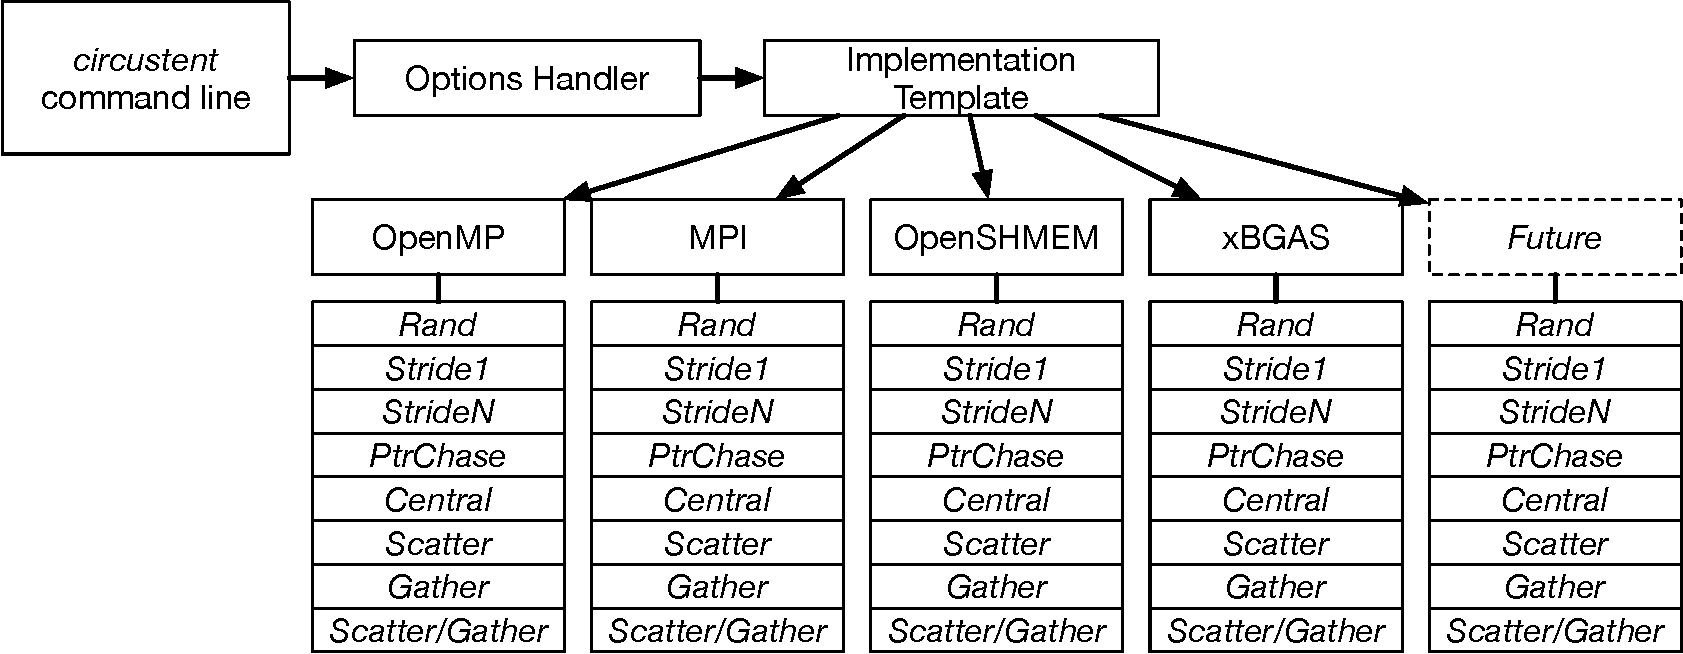
\includegraphics[width=5in]{figures/arch.pdf}
\caption{CircusTent Architecture}
\label{fig:ct_arch}
\end{figure*}

%\todo[inline]{I'd suggest to classify related work into a few categories and have a sub-section for each category to make the organization and presentation better structured. -Yong}
% Done - Brody

\subsection{Atomic Operations \& Synchronization}
\label{subsec:amos_sync}

Several previous studies have examined the behavior and performance characteristics of atomic operations and synchronization primitives.
Villa et al. explored the efficiency and scalabilty of barrier based synchronization on manycore architectures utilizing intraprocessor interconnects modeled after the design of network-on-chip (NOC) paradigms \cite{villa2008barriers}.
In this study, the authors evaluated four different barrier algorithms, implemented in both hardware and software, using a cycle-accurate simulator.
Trials conducted using up to 128 cores, arranged in five different topologies, revealed that, at least for similar configurations, hardware based barrier implementations exhibit better performance for intraprocessor synchronization.

In a similar study, David et al. conducted an extensive investigation of synchronization that spanned multiple hardware and software methodologies \cite{david2013sync}.
Based on the results of their evaluation, the authors of this work made several important observations.
First, they note that, regardless of the implementation, synchronization across sockets is far more expensive than intrasocket synchronization.
In fact, even in the absence of contention, the authors found that the latency of operations performed on cache lines across sockets increased 2-7.5x as compared to their intrasocket analogs.
Second, they observe that the organization and behavior of the of the last-level cache (LLC) plays an important role in synchronization scalability within a socket.
Finally, they perceive that, as the number of threads contending for access to shared data grows, message-passing mechanisms often outperform locking schemes.
Overall, for physically shared memory systems such as those utilized in this work, the authors conclude that the scalability of synchronization is directly correlated to the system's architecture.

In \cite{schweizer2015evaluating}, Schweizer et al. develop a methodology for analyzing the latency and bandwidth of atomic operations.
In particular, they study the effects of different cache coherency states and complex memory hierarchies on these operations.
Using their proposed methodology, they then evaluate three different RMW atomic operations on a number of x86 platforms.
As part of this evaluation, they show that, contrary to popular belief, all of the tested atomic operations exhibit comparable performance in terms of latency and bandwidth.
Further, they find that, even in the absence of dependencies between instructions, the design of atomic operations on the tested platforms inherently prevents instruction-level parallelism.

Hoseini et al. also study the properties of atomic operations in physically shared memory systems \cite{hoseini2019modeling}.
For their investigation, they monitor accesses to shared cache lines in conditions that simulate both high and low levels of contention.
Notably, for the high contention environment, wherein requests to a single cache line become serialized, they examine the scheduling of thread accesses.
For one platform utilizing a Xeon-E5 processor, they were unable to discern any deterministic scheduling pattern.
However, for the other platform featuring a Knights Landing Xeon Phi processor, they observe that threads pinned to cores coresident on the same tile were always scheduled sequentially.
This is logical as this processor employs L2 caches that are shared between cores on the same tile, but does not include an LLC shared between all cores.

Although each of the studies detailed above make important contributions and advance our understanding of atomic operations and synchronization primitives, they do so only in a limited number of carefully controlled scenarios.
As such, the behaviors and performance characteristics they observe may not be fully generalizable to varied architectures and applications.
Furthermore, the specialized approaches they employ are applicable only for physically shared memory systems and not easily replicated.
In contrast, CircusTent provides an infrastructure for benchmarking the performance of atomic operations that is built directly on conventional shared and distributed shared memory parallel programming models.
In this manner, CircusTent offers an easily accessible, uniform means of measuring memory subsystem performance in common application environments across diverse platforms.

\subsection{Transactional Memory}
\label{subsec:trans_mem}

Transactional memory (TM) represents an orthogonal approach to synchronization that has become increasingly prominent in recent years.
Similar to the use of atomic operations, this paradigm seeks to avoid the performance overheads associated with lock-based synchronization.
However, it targets concurrent accesses to shared data at a more coarse-grained level. 
Rather than operating on a single value, as with an atomic operation, this approach encapsulates a series of instructions into a ``transaction".
In many ways, these transactions correspond to critical code segments traditionally protected using lock-based synchronization.
In contrast, however, simultaneous accesses to the data underlying a transaction by distinct processing elements is not inherently prevented.
Instead, operations on this data are speculatively performed and tracked across processing elements.
In the absence of a conflict, changes to the data are committed.
If a conflict is detected, these changes are discarded instead.
In this manner, transactional memory represents an optimistic approach to synchronized data access in a parallel environment.

Previous studies have implemented transactional memory in both hardware and software.
Hardware Transactional Memory (HTM) was originally proposed by Herlihy and Moss \cite{herlihy1993lockfree}.
In this first work on transactional memory, the authors exploited access right policies within existing cache coherency protocols to realize their implementation.
This implementation added new ISA-level instructions, as well as a distinct \textit{transactional cache}, to enable hardware-level support for the paradigm.
Locations accessed within the scope of a transaction by these new transactional load and store variants were traced using an associated \textit{read set} and \textit{write set}, respectively.
Ananian et al. described and developed an extension to HTM that allows transactions to scale to near virtual memory levels through the use of a memory-resident logging structure \cite{ananian2006unbounded}.

Software Transactional Memory (STM) was first demonstrated by Shavit and Touitou \cite{shavit1995softwaretm}.
The methodology detailed in this work provided the capabilities of non-blocking transactional memory to existing systems at the software level through the utilization of only standard load-linked and store-conditional ISA instructions.
Moreover, it also introduced the concept of helper policies for transactions between processing elements.
This initial implementation was, however, only applicable to static transactions that accessed a predetermined sequence of memory locations.
This limitation was largely overcome in a subsequent work by Herlihy et al. \cite{herlihy2003stmdsds}.
Bocchino et al. further expanded the notion of STM and developed the first implementation targeted towards Partitioned Global Address Space models in distributed memory environments \cite{bocchino2008stm}.
Herein, the authors found that, when utilized in conjunction with the GASNet library, their implementation was able to efficiently scale to up to 512 processors.
In addition to standalone HTM and STM methodologies, some studies have also sought to couple the performance of HTM together with the extensiblilty of STM in a hybrid approach \cite{baugh2008using}.

An in-depth comparison of transactional memory and atomic-based synchronization is beyond the scope of this work.
However, it is worth noting that utilization of HTM is limited to systems with underlying microarchitecural support.
Further, lock-based synchronization cannot always be directly translated to analagous transactional memory routines \cite{blundell2006subtleties}.
As such, the performance of atomic operations and associated synchronization primitives will be of continued importance to future systems.

\subsection{Memory Benchmarks}
\label{subsec:memory_bench}

The Spatter Benchmark, developed by Lavin et al., is also directly relevant to this work \cite{lavin2018spatter}.
Although Spatter does not analyze the performance of synchronization primitives or atomic operations, similar to CircusTent, it is designed to benchmark the memory hierarchies of target architectures.
More specifically, Spatter measures an architecture's memory performance with respect to an emerging class of indexed memory access patterns known as scatter and gather operations.
Highly tunable, Spatter provides an efficient means of measuring these irregular, non-uniform memory access patterns increasingly common to HPC applications in a manner previous existing benchmarks could not.
Currently, Spatter supports both OpenMP and CUDA backend implementations for both CPU and GPU-based platforms.
As detailed in Section~\ref{subsec:algorithms}, CircusTent also integrates kernels that replicate these memory access patterns, but does so using atomic operations in lieu of traditional loads and stores.

%\todo[inline]{Possibly add transactional memory papers depending on space}
%\todo[inline]{I'd suggest to add TM discussion please, as reviewers would expect this discussion and a comparison when we discuss AMOs. -Yong}
% Done - Brody
